\documentclass[a4paper,11pt]{article}

\usepackage[ansinew]{inputenc}
\usepackage[french]{babel}
\usepackage[T1]{fontenc}
\usepackage[paper=a4paper, top=1cm, bottom=1cm, left=2cm, right=2cm]{geometry}
\usepackage{graphicx}
\usepackage{hyperref}
\usepackage{url}
\usepackage{xcolor}

\title{\large{\bfseries{ARCHITECTURE LOGICIELLE}}}
\author{Beno\^it V\'edrenne, Gaël Walter}

\begin{document}

\maketitle

\begin{center}
\emph{Charg\'e de TD :} Damien Cassou\end{center}

\vspace{0.5cm}

\begin{center}

\includegraphics[width=2.5cm,height=2.5cm]{images/bdx1.eps}\\
\large{Universit\'e Bordeaux 1,\\
351 cours de la Lib\'eration,\\
33405 Talence Cedex,\\
France}
\end{center} 

\vspace{0cm}

\begin{center}
 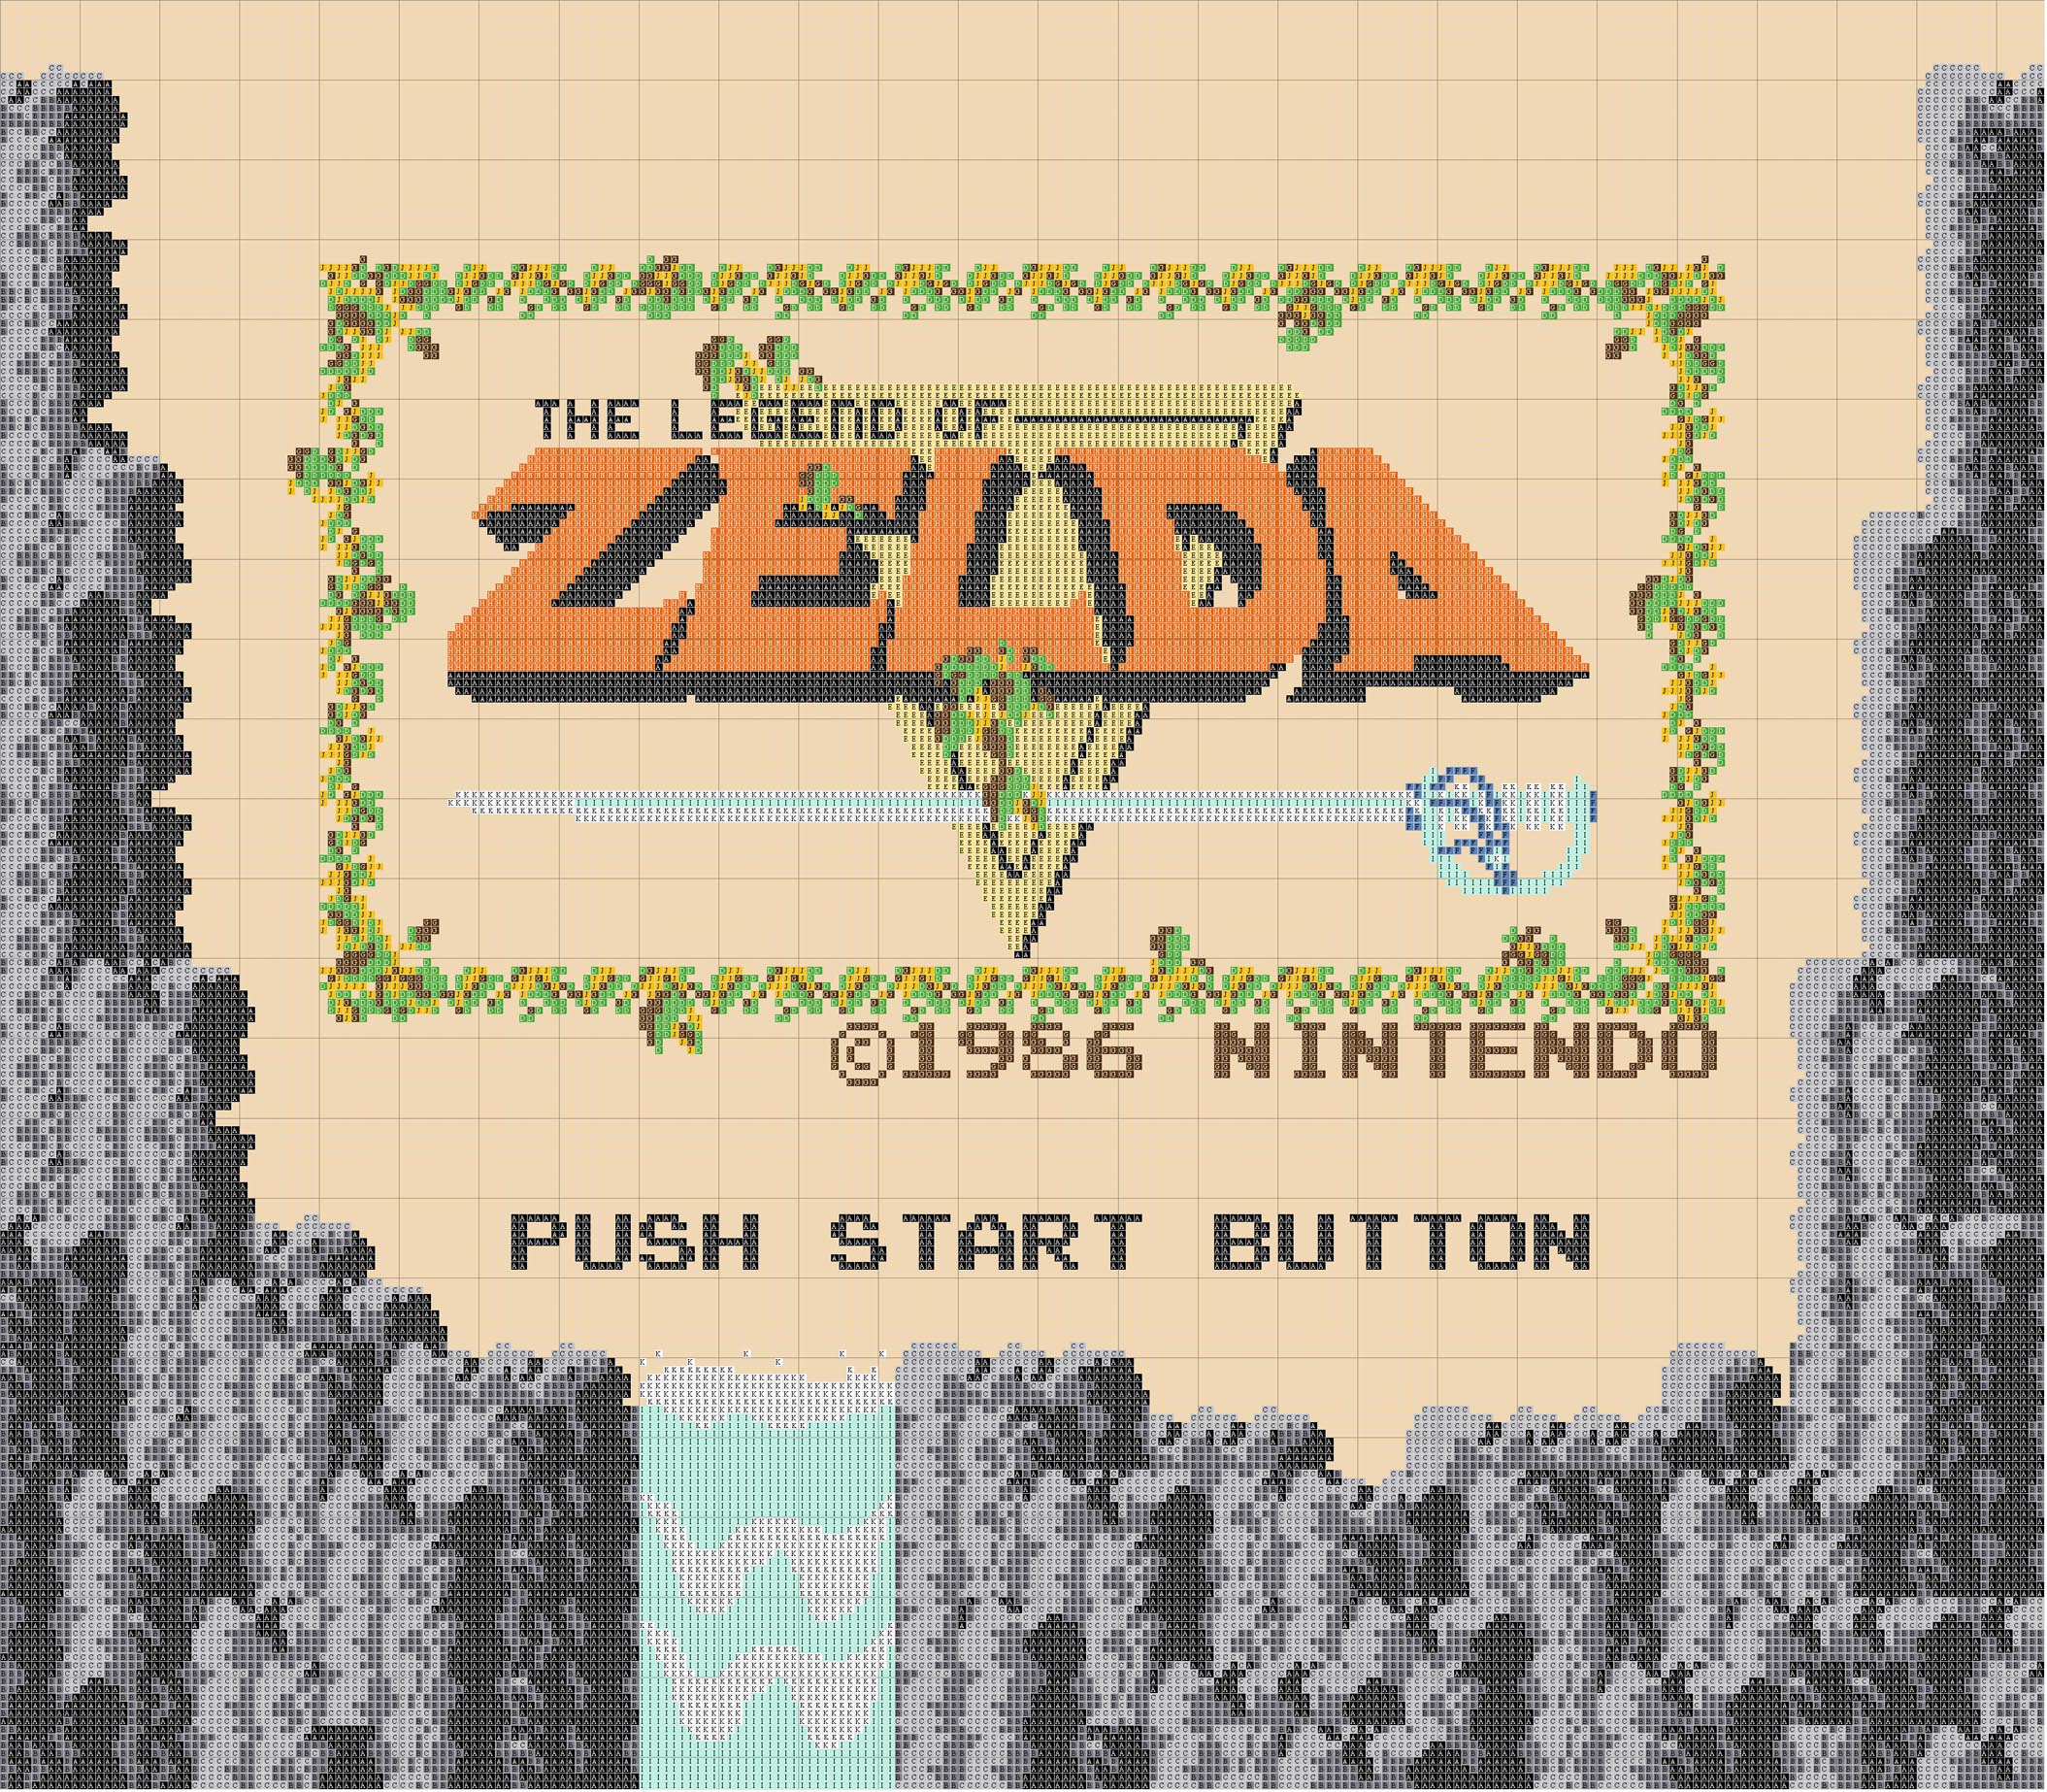
\includegraphics[width=9cm,height=9cm]{images/zeldaNintendo.eps}
\end{center}

\begin{center}
 \large{The Cremi Legend Of Zelda}
\end{center}

\begin{abstract}
La l\'egende raconte que la grande for\^et d'Hyrule est occup\'ee par Ganon, le
puissant Prince des T\'en\`ebres. Ganon a captur\'e la fille du Roi qui tenta de s\'eparer la
Triforce, puissant sortil\`ege qui prot\`ege le royaume d'Hyrule. Ses guardes
mal\'efiques avancent \`a grand pas dans la for\^et en d\'etruisant tout sur leurs
passages\ldots \\
Il existe cependant un chevalier courageux, en ces temps de manants. 
On le reconnait facilement \`a sa chevelure blonde sous sa longue cape
verte. Apprenant la nouvelle de l'invasion, le regard noir,
il parti dans les haut bois de la for\^et d'Hyrule pour les affronter tous et
lib\'erer la fille du Roi nomm\'ee ``Zelda''.\\

The ``CREMI Legend of Zelda'', c'est l'histoire de ce jeune garçon, nomm\'e
LinkAuber, alias Link qui doit sauver la princesse Zelda au p\'eril de sa vie. \\
Une somme d'embûches l'attend. L'art de manier son \'ep\'ee pourra peut \^etre
l'aider dans sa qu\^ete impossible: seul contre une arm\'ee enti\`ere.
\end{abstract}

\newpage

\section{Introduction}
Le framework de jeu plateforme dont nous disposions, nous a permis
d'impl\'ementer une version du Jeu Zelda. Ce jeu, cr\'e\'e par Miyamoto (auteur
\'egalement de Donkey Kong et Mario), poss\`ede une version Nintendo de 1986. \\

Notre application s'inspire de cette version l\`a, o\`u l'on peut guider dans une
for\^et le personnage Link. Il peut utiliser son \'ep\'ee avec la touche ``Espace'', comme notre version. \\
Nous l'avons bien sûr d\'enomm\'e Cremi Legend Of Zelda car il a \'et\'e principalement
d\'evelopp\'e au Cremi !

\subsection{Comment jouer \`a CLOZ ?}
Le but du jeu est de guider Link dans la for\^et pour l'amener \`a la
princesse Zelda avec les
touches fl\'ech\'ees. \\ 
On devra tout d'abord \'eliminer tout ses ennemis mal\'efiques en utilisant le coup
d'attaque par la touche ``Espace''. Ceux ci sont tr\`es \'enerv\'es car
ils ont \'et\'e pr\'evenus de l'arriv\'e de Link, c'est pour cela qu'ils n'ont pas un
comportement tr\`es logiques. Parfois, il se peut qu'un ennemi plus robuste
surveille plus raisonnablement Zelda, il est donc plus difficile \`a
tuer. Il ne faut pas h\'esiter \`a les frapper de manière r\'ep\'et\'ee.\\

La difficult\'e du jeu r\'eside dans le nombre d'ennemis \`a tuer, plus ou moins
forts selon leurs grades, mais aussi dans les diff\'erents objets
qui peuvent agr\'ementer le jeu. Le joueur est libre de tous les
essayer. Mais comme dans la r\'ealit\'e, les bombes, ça fait mal.\\

La vie de Link d\'emarre \`a ``100'' mais elle peut descendre tr\`es
vite ! Faites attention Link, n'est pas immortel. En mourrant, vous
recomancez le jeu au d\'ebut du niveau.

\subsection{Quelques r\`egles du jeu}
Seul le clavier est utile au jeu, mais le menu permet d'autres actions.\\
Au croisement avec des ennemis, Link perd de la vie car il se fait
frapper par ceux-ci. Les boss sont de vrai brute, ils tapent fort. Si
notre h\'eros meurt, le niveau de
jeu red\'emarre au d\'ebut. \\
Depuis le menu, on peut red\'emarrer la partie au d\'ebut, mais aussi sauvegarder la
partie ou (en th\'eorie) en restaurer une.\\
Lorsque tout les ennemis sont tu\'es, il faut aller vers la princesse et le
niveau est gagn\'e, on passe alors automatiquement au niveau suivant, s'il existe.
On peut trouver une arme sur le sol, Link peut attaquer avec. Il est possible
que certaines actions enl\`eve cette arme, et la le combat de boss est
plus difficil. 

\subsection{Astuces}
Comme dans beaucoup de jeu vid\'eo d'aventure, nous avons laiss\'e des codes
secrets que l'on peut chercher si l'on veut. Qu'il est agr\'eable en \'etant joueur
de trouver ce genre de code ! Mais n'oubliez pas que l'abus de code nuit
au plaisr de jouer.

\newpage

\section{Conception}

\subsection{Pacquetages}
Le paquetage ``\textbf{zelda}'' comprend plusieurs paquetages.\\
Le paquetage ``\textbf{base}'' permet de g\'erer l'interaction utilisateur, sons,
gestion de mouvements de personnages.\\ 
Le paquetage ``\textbf{rule}'' permet de
g\'erer les collisions ou blocages entre entit\'es du jeu.\\ 
Le paquetage
``\textbf{level}'' permet de g\'erer la mise en place des niveaux du jeu, de la
lecture de fichier pour les niveaux, \`a la cr\'eation de niveaux.\\ 
Le paquetage
``\textbf{game}'' contient les classes n\'ecessaires \`a la cr\'eation du jeu
(gestion de l'univers, sauvegarde de niveaux\ldots).\\ 
Le paquetage
``\textbf{observer}'' permet de g\'erer tout les observateurs du jeu.\\ 
Le paquetage ``\textbf{entity}'' poss\`ede toutes les classes de toutes les entit\'es 
pr\'esentes dans le jeu : personnages et d\'ecors. Dans les personnages, un paquetage 
est r\'eserv\'e aux \'etats de Link.\\

\subsection{Architecture g\'en\'erale}

\begin{center}
 %\includegraphics[width=9cm,height=9cm]{images/archiGenerale.eps}
\end{center}

\subsection{Architecture d\'etaill\'ee}

\subsubsection*{Une Fabrique Abstraite pour cr\'eer le niveau depuis un fichier
texte}
Nous avons choisi d'utilis\'e une fabrique abstraite pour permettre la
cr\'eation et l'ajout d'entit\'e dans le niveau. Il \'etait assez interressant
de cr\'eer cette fabrique abstraite car aisni nous faisions juste une
demande de cr\'eation d'un certain objet \`a celle-ci et elle s'occuper du
reste. Une personne voulant cr\'eer un personnage ou une autre entit\'e a
juste besoin de faire appel \`a la m\'ethode create ad\'equate. Cependant, le
probl\`eme le plus important et qui est un probl\`eme propre \`a ce mod\`ele,
c'est que l'ajout de nouvelles entit\'es est assez fastidieux.

\begin{center}
 %\includegraphics[width=9cm,height=9cm]{images/abstFab.eps}
\end{center}

\subsubsection*{Le pattern Monteur pour sauvegarder la partie}
Le fait de sauvegarder la partie est une action classique de tout
jeu. Il nous est apparu comme \'evident d'avoir une repr\'esentation sur
fichier du contenu de cette sauvegarde. Nous avons donc mis en place un
monteur, celui-ci en effet est particuli\`erement adapt\'e \`a ce genre de
situation. Nous avons donc cr\'eer un monteur concret qui permet d'\'ecrire
un fichier texte contenant les informations ainsi sauvegarder.\\
Un autre avantage de ce patron de conception est que nous pouvons ainsi
rapidement modifier la repr\'esentation de cette sauvegarde. Il est tout \`a
fait possible d'imagin\'e une sauvegarde au format HTML ou XML, ou on ne
sait quel autre format. Le format de la sauvegarde est donc facilement
modifiable pour n'importe quelle personne reprennant notre code et qui
n'aimerait pas notre repr\'esentation. \\

\begin{center}
 %\includegraphics[width=9cm,height=9cm]{images/monteur.eps}
\end{center}

Nous avons aussi utilis\'e ce mod\`ele pour la lecture de la sauvegarde
ainsi que la lecture du fichier de cr\'eation de niveau et ce pour les
même raison que celle \'enonc\'e juste avant.

\subsubsection*{Gestion des \'etats de Link avec le pattern Etat}
L'\'etat de Link modifie son comportement. Ces changements
apparaissent de façon dynamique, selon les \'evenements du jeu, ou du joueur.
Cette intention nous a amen\'e \`a utiliser le pattern Etat pour g\'erer Link. Celui
ci peut d\'el\'eguer son comportement changeant \`a une hi\'erarchie de classes
LinkState poss\'edant des requ\^etes sp\'ecifiques comme l'utilisation de l'arme, le
mode attaque, la mort du personnage\ldots
Sur la fin du d\'eveloppement, cette conception nous a permis de rajouter
rapidement de nouveaux \'etats, et d'ajuster le comportement voulu facilement. \\

\begin{center}
 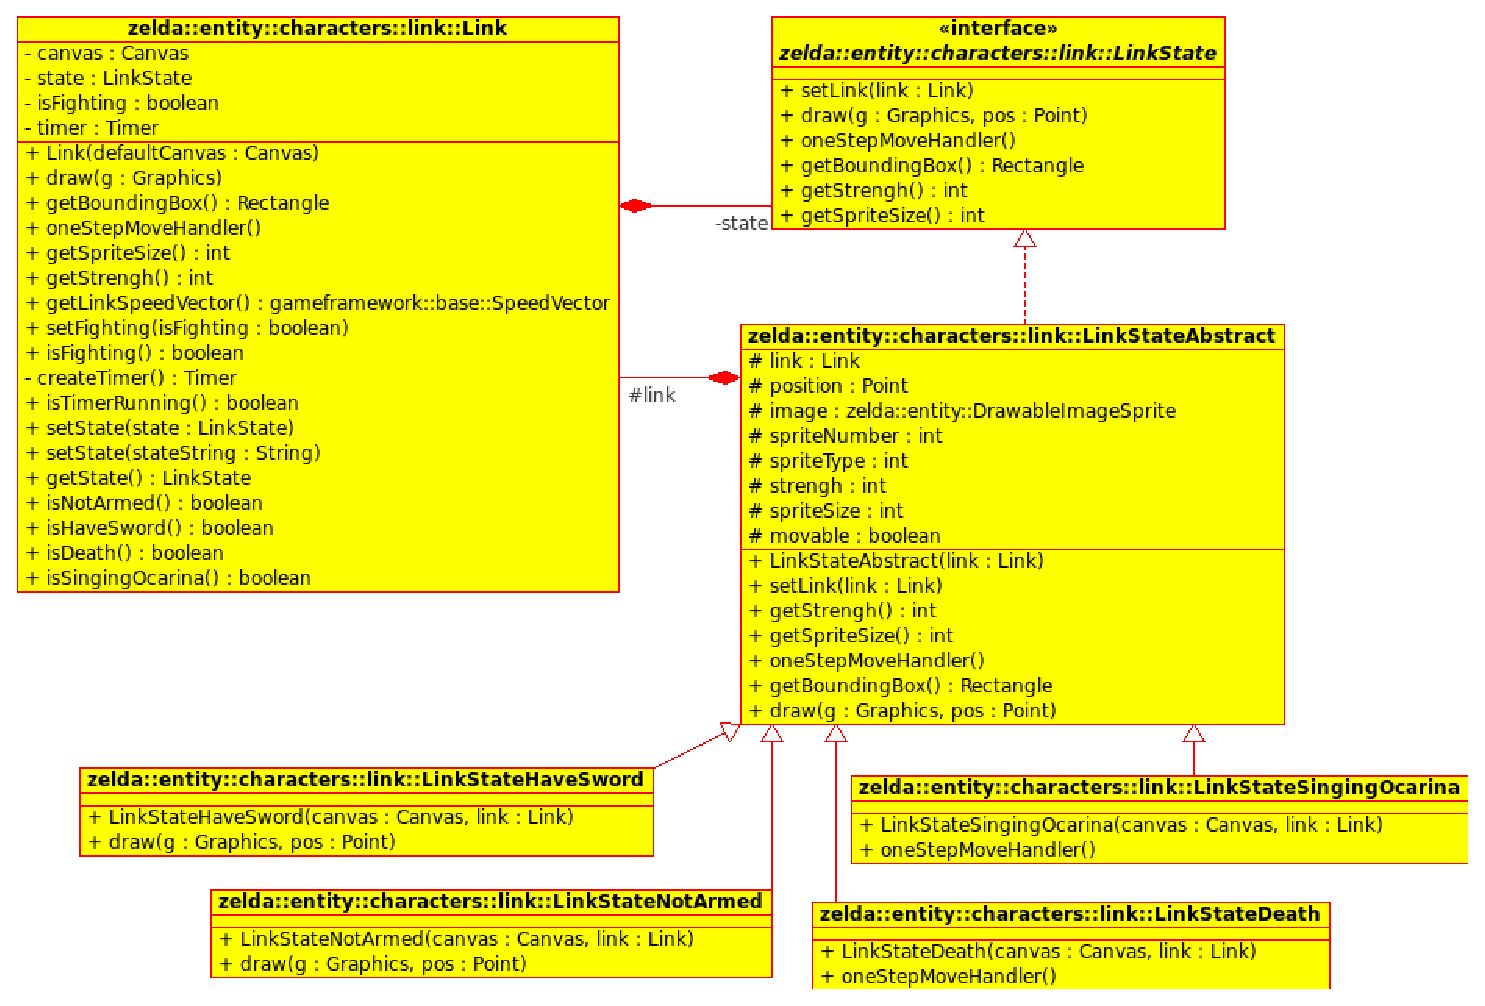
\includegraphics[scale=0.8]{images/Statediagram.eps}
\end{center}
 
\subsubsection*{Gestion du niveau avec des observateurs}
 
\end{document}
